\documentclass[11pt]{article}
\usepackage[hmargin=1.13in,vmargin=1.05in]{geometry}
\usepackage{amsmath,amssymb,amsthm,booktabs}
\usepackage{microtype,tikz}
\usepackage[hidelinks,pdfusetitle]{hyperref}
\newtheorem{theorem}{Theorem}
\newtheorem{lemma}[theorem]{Lemma}
\theoremstyle{remark}
\newtheorem*{example}{Example}
\newcommand{\ar}{\operatorname{ar}_{\mathbb C}}
\newcommand{\mr}{\operatorname{mr}}
\newcommand{\br}{\operatorname{br}}
\newcommand{\Ext}{\operatorname{Ext}}
\newcommand{\cl}[1]{\widehat{#1}}
\newcommand{\port}[2]{#1.#2}
\title{Prime Knots with Augmentation-Rank Gaps\\ at Unbounded Bridge Number}
\author{Roy van Rijn}
\date{}

\begin{document}
\maketitle

\begin{abstract}
We construct explicit braid families containing infinitely many distinct
hyperbolic prime knots of each bridge number \(b=5,6\) and each sufficiently
large \(b\), with complex augmentation rank at most \(b-1\) and meridional
rank \(b\). Alternating-group colorings force \(b\) meridional generators,
while two fixed meridian words let a local rank-one obstruction
persist as the braid grows. An oriented diagram isotopy realizes the
associated two-cusped exteriors as fillings of a single three-cusped
exterior. Rigorous interval certificates establish
hyperbolicity of that exterior and the two small-bridge exteriors used
in the filling argument.
\end{abstract}

\section{Introduction}

How far can one get in determining the bridge number of a knot using
rank-one meridian representations? For a knot \(K\subset S^3\), the
meridional rank \(\mr(K)\) is the least number of positive meridians
generating its group, and the bridge number \(\br(K)\) is the least
number of maxima in a bridge presentation. The conventional complex
augmentation rank \(\ar(K)\) uses the cord algebra with \(U=1\) and
meridian parameter different from \(1\). By Cornwell's correspondence it
is the maximum dimension of an irreducible complex representation in
which a meridian is diagonalizable with eigenvalues \(1,\ldots,1,\mu\),
where \(\mu\ne 0,1\) \cite[Theorem 1.2 and Definition 1.8]{Cornwell}.
Meridians are conjugate, so this condition holds for every meridian.
The inequalities
\[
                 \ar(K)\le \mr(K)\le\br(K)
\]
give two ways to bound bridge number from below. We construct prime
knots of arbitrarily large bridge number for which the first bound
falls short and the second is an equality.

Read braid words from left to right, from top to bottom, and write
\(\sigma_i\) for the positive crossing at positions \(i,i+1\).
Let
\[
 U=\sigma_1\sigma_2\sigma_3^{-2}\sigma_2\sigma_3^{-2}
          \sigma_2\sigma_1^2\sigma_2^3\sigma_3^{-1}\in B_4.
\]
For \(b\ge5\), put \(d=b-2\) and embed \(U\) in \(B_b\) on the first
four strands. Define
\[
 \delta_b=\sigma_2(\sigma_3\sigma_4\sigma_3^{-1})
                  \sigma_5\cdots\sigma_{b-1},\qquad
 K_{b,k}=\cl{U\delta_b^{(d+1)(1+d^2 k)}}\quad (k\ge0).
\]
An empty product is the identity.

\begin{theorem}\label{thm:main}
For every integer \(b\ge5\) and \(k\ge0\), \(K_{b,k}\) is a knot and
\[
              \ar(K_{b,k})\le b-1<\mr(K_{b,k})=\br(K_{b,k})=b.
\]
For each \(b=5,6\) and each sufficiently large \(b\), all sufficiently
large \(k\) give hyperbolic prime knots, and infinitely many distinct
knot types occur for that fixed \(b\).
\end{theorem}

Cornwell proved \(2=\ar(K)<\mr(K)=3\) for the four knots
\(8_{16},8_{17},10_{91},10_{94}\) and their mirrors. His rank-gap
classification assumes crossing number at most ten and bridge number
and braid index both equal to three, and its augmentation upper bounds
use Gröbner bases of braid-specific equations
\cite[Corollary 1.12 and Theorem 5.3]{Cornwell}. Theorem~\ref{thm:main}
gives infinite hyperbolic prime families at unbounded bridge number.
Gao, Gu, Li and Wang prove \(\ar\le5<\mr=\br=6\) for the
untwisted Whitehead double of the square knot, using its satellite
presentation for the augmentation bound and a finite quotient and
cocycle calculation for the meridional bound
\cite[Theorem 1.3 and Section 6]{GGLW}.
Here the rank-one obstruction persists under a family of braid tails,
and the diagram isotopy produces hyperbolic examples without taking
satellites or connected sums. The theorem gives an upper
bound on augmentation rank. Its hyperbolicity cutoffs are existential,
and the cutoff in \(k\) is allowed to depend on \(b\).

The algebraic construction uses the same braid action in two ways.
The braid after \(U\) fixes the first and fourth meridians. After
conjugating the labels on strands five through \(b\) by the fourth
label, this part of the braid acts by ordinary Hurwitz moves on the
remaining entries. These moves preserve their ordered product. In an
alternating group we can compute the order of this product explicitly
and use it to close up a coloring that needs \(b\) generators. In a
rank-one representation, assuming that both the displacement vectors
and their covectors are independent forces two matrix identities inside
\(U\). Seven signed crossing relations then give a contradiction.

The two filling steps use different peripheral markings. The first
filling uses the disk marking of a cusp of the fixed three-cusped
exterior. The homeomorphism to the two-cusped parent is unmarked
and transfers hyperbolicity. The second filling uses the original
disk marking of the circle in that parent.

To obtain the two-cusped parent, put a circle around the strands
carrying the Hurwitz moves. Varying \(k\) amounts to filling that
circle. The number of strands through it varies with \(b\), so a separate
argument is needed to control the exteriors before filling. The
diagram isotopy in Section~\ref{sec:geometry} trades each extra
threaded curl for a full twist between a knot arc and a circle arc.
This identifies all the two-cusped exteriors with fillings of a
single three-cusped manifold, to which we apply hyperbolic Dehn
filling twice.

\section{Alternating-group colorings}\label{sec:color}

For any group, the Wirtinger rule at a positive braid crossing is
\(T(a,c)=(c,c^{-1}ac)\); its inverse is
\(T^{-1}(a,c)=(aca^{-1},a)\). A tuple of labels at the top of a closed
braid defines a homomorphism from the knot group exactly when the
crossing rules return the tuple at the bottom. The image is generated
by the top labels, because they generate the Wirtinger group.

Put \(g=\sigma_3\sigma_4\sigma_3^{-1}\).
On the entries \((a,C,e)\) at positions \(3,4,5\), its action is
\[
                 (CeC^{-1},\,C,\,e^{-1}C^{-1}aCe).
\]
In particular, \(g\) fixes the fourth label and acts as \(T\) on
\((a,CeC^{-1})\). The subgroup of \(B_b\) generated by
\(\sigma_2,g,\sigma_5,\ldots,\sigma_{b-1}\) fixes entries one and
four and acts by adjacent Hurwitz moves on the tuple
\begin{equation}\label{eq:framed}
                  (M_2,M_3,CM_5C^{-1},\ldots,CM_bC^{-1}),
                  \qquad C=M_4.
\end{equation}
This follows for the last generators because simultaneous conjugation
commutes with \(T\), and then holds for inverses as well. The product of
the entries in \eqref{eq:framed} is invariant, since \(T(a,c)\) has
product \(ac\).

We use permutations composed from right to left. The top labels on
\(2b\) symbols are
\[
\begin{aligned}
 x_0&=(0\,1)(2\,3), &x_1&=(1\,4)(2\,3),\\
 x_2&=(0\,5)(1\,6), &x_3&=(1\,2)(6\,7),\\
 x_4&=(0\,8)(7\,9), &
 x_j&=(2j-2\,\,2j)(2j-1\,\,2j+1)\quad(5\le j<b).
\end{aligned}
\]
The first four generate \(A_8\). Indeed, \(x_0x_1\) is a
three-cycle on \(\{0,1,4\}\). By conjugating that cycle by \(x_2\)
and \(x_3\), then conjugating the resulting cycles by \(x_3\) and
\(x_0\), respectively, we obtain the additional supports
\[
       \{4,5,6\},\quad \{0,2,4\},\quad \{4,5,7\},\quad \{1,3,4\}.
\]
These cycles generate \(A_8\). To see the enlargement at each step,
an alternating group on an old set of at least three symbols together
with a three-cycle on two old symbols and one new symbol generates
the alternating group on the union. Conjugations and inverses give
both orientations for every pair of old symbols, including when the
old set has size three. If the cycle has just one old symbol,
conjugate it by an old permutation moving that symbol. The product
of the original cycle with the inverse conjugate gives a cycle on
two old symbols and one new symbol, after which the other new
symbol can also be added. The displayed supports can therefore be
adjoined in order. Each \(x_j\) for \(j\ge4\) consists of two
transpositions \((a\,u)(c\,v)\) with distinct old symbols \(a,c\)
and distinct new symbols \(u,v\). Conjugate it by an even old
permutation fixing \(c\) and moving \(a\), and multiply the
two double transpositions. This gives a three-cycle on two old
symbols and \(u\). Repeat with \(a,u\) fixed and \(c\) moved to
adjoin \(v\). The full tuple generates \(A_{2b}\).

To check the coloring, let \(X=x_1,\ Y=x_2,\ C=x_3\).
Applying the crossing rule through \(U\) gives
\[
       (x_0,a,h,C,x_4,\ldots,x_{b-1}),\qquad
       a=(0\,5)(1\,4),\quad h=(1\,6)(2\,3).
\]
This four-strand calculation can also be read from the crossing
relations in \eqref{eq:prefix}. With \(z_i=Cx_{i+3}C^{-1}\) for
\(1\le i\le d-2\), the product of the middle tuple
\((a,h,z_1,\ldots,z_{d-2})\) is
\[
 p=(0\,8\,10\,\cdots\,2b-2\,\,5)
   (1\,6\,9\,11\,\cdots\,2b-1\,\,4)(2\,3).
\]
In each displayed progression the terms run only up to the indicated
endpoint. For \(b=5\) the product is the one computed below.
For larger \(b\) each additional factor inserts its two new
symbols just before \(5\) and \(4\) in the respective cycles.
The two long cycles have lengths \(d\) and \(d+1\), so
\(p\) has order \(d(d+1)\). Reading the cycles gives
\[
        pXp^{-1}=h,\qquad
        p^iYp^{-i}=z_i\ (1\le i\le d-2),\qquad p^dYp^{-d}=a.
\]
The adjacent moves in \(\delta_b\) act on \eqref{eq:framed} as the
left shift that sends the first entry \(m\) to \(p^{-1}mp\) at the
end. After \(d\) shifts all labels have been conjugated by \(p^{-1}\).
After \(d+1\) shifts the three displayed identities return the initial
middle tuple \((X,Y,z_1,\ldots,z_{d-2})\). Adding
\(d^2(d+1)k\) shifts has no effect because \(p\) has order \(d(d+1)\).

\begin{example}
At \(b=5\) the middle tuple has length three and
\(p=(0\,8\,5)(1\,6\,9\,4)(2\,3)\). Four shifts close the
coloring of \(U(\sigma_2g)^4\), and a further \(36\) shifts act
trivially. This gives the exponent \(4+36k\) on five strands.
\end{example}

The strand permutation of \(\delta_b\) is a \(d\)-cycle on positions
\(\{2,3,5,\ldots,b\}\); its exponent is \(1\bmod d\).
The permutation of \(U\) is \((1\,2)(3\,4)\). The two transpositions
insert the two omitted positions into that cycle, giving one knot
component. Its group surjects onto \(A_{2b}\) by the coloring just
constructed. A double transposition moves two independent directions in the natural
permutation representation over \(\mathbb C\). The following lower
bound uses its two transposition edges. A set of at most \(b-1\) double transpositions has a
support graph with at most \(2b-2\) edges on \(2b\) vertices. Each
generator preserves the components of the graph, so such a set
cannot generate a transitive group. The quotient forces
\(\mr(K_{b,k})\ge b\), since every positive meridian is conjugate to
a top label. A closed \(b\)-strand braid gives a bridge presentation
with at most \(b\) maxima, and the Wirtinger relations of a bridge
presentation give one generating meridian per bridge. Thus
\(\mr(K_{b,k})=\br(K_{b,k})=b\).

\section{The rank-one obstruction}\label{sec:rank}

We prove an upper bound for every knot obtained by following \(U\)
with a braid in the subgroup acting on \eqref{eq:framed}. That
subgroup fixes the first and fourth meridian words. These two fixed
positions suffice for the rank-one argument.

\begin{lemma}\label{lem:spans}
Suppose that \(\tau\) belongs to
\(\langle\sigma_2,g,\sigma_5,\ldots,\sigma_{b-1}\rangle\) and
\(\cl{U\tau}\) is a knot. Let its group act on a finite-dimensional
space \(V\) over a field so that each meridian has displacement
of rank one. Write each meridian as \(M=I-u f\), where \(u\in V\)
and \(f\in V^*\). Then at least one of the spans of all the \(u\)'s
and all the \(f\)'s has dimension at most \(b-1\), and both
dimensions are at most \(b\).
\end{lemma}

\begin{proof}
Each of the two spans is already spanned by its \(b\) top-strand
vectors or covectors. The root span of the generating meridians is
invariant under those generators and their inverses, and the
covector span is invariant under right multiplication by the same
matrices. Conjugating a generator therefore introduces neither a
new root direction nor a new covector direction.

Suppose both spans have dimension \(b\). In particular both
families of four vectors and covectors on the first four strands
are separately independent. Set
\[
 \mu=\det M\ne0,\qquad f(u)=1-\mu,\qquad
 M^{-1}=I+\mu^{-1}u f.
\]
The first two identities hold for every meridian, with one common
\(\mu\). When \(M_a=I-u_a f_a\), conjugation by a matrix \(J\)
replaces its pair by \((Ju_a,f_aJ^{-1})\). Two pairs for the same
nonzero displacement differ by reciprocal scaling.

Here is the crossing trace through \(U\). We use arc subscripts on
the matrices \(M_i\) in this proof. A row \((o,a,c,\epsilon)\)
represents \(M_c=M_o^\epsilon M_aM_o^{-\epsilon}\).
The input labels are \((1,0,8,13)\) and the output labels are
\((1,6,16,13)\).
\begin{equation}\label{eq:prefix}
\begin{array}{c|rrrr@{\qquad}c|rrrr}
0&0&1&2&-&1&8&2&3&-\\
2&3&13&14&+&3&14&3&4&+\\
4&4&8&9&-&5&9&14&15&+\\
6&15&9&10&+&7&10&4&5&-\\
8&10&0&1&-&9&1&10&11&-\\
10&5&11&12&-&11&12&5&6&-\\
12&6&12&13&-&13&13&15&16&+
\end{array}
\end{equation}
The repeated outer labels express closure, since \(\tau\) fixes
the first and fourth entries. Each row is obtained by \(T\) or
\(T^{-1}\) in the order of the letters in \(U\).

Put \(A=M_2,\ B=M_8,\ C=M_{13},\ D=M_0\).
Replacing \(M_1\) by \(A=D^{-1}M_1D\) changes the root by a
multiple of the root of \(D\) and the covector by a multiple of
its covector, preserving both independent families.
Let \(H\) and \(F\) denote the root and covector spans of
\(A,B,C\), respectively. Both have dimension three, and in the
pair \((v,\nu)\) of \(D\) one has \(v\notin H\) and \(\nu\notin F\).
Rows \(1\) through \(7\) and row \(13\) propagate pairs in \(H,F\).

Rows \(0\) and \(8\) give \(DAD^{-1}=X^{-1}DX\) for
\(X=M_{10}\). If \(A,X\) have pairs \((a,f)\) and \((x,\xi)\)
in \(H,F\), comparing the pairs on both sides gives
\[
 \begin{aligned}
 a-\nu(a)v &= \lambda\bigl(v+\mu^{-1}\xi(v)x\bigr),\\
 f+\mu^{-1}f(v)\nu &= \lambda^{-1}\bigl(\nu-\nu(x)\xi\bigr)
 \end{aligned}
\]
for some \(\lambda\ne 0\). The coefficients on \(v,\nu\)
give \(\lambda=-\nu(a)\) and \(f(v)=\mu\lambda^{-1}\).
The other components give
\(a=\lambda\mu^{-1}\xi(v)x\) and \(f=-\lambda^{-1}\nu(x)\xi\).
Applying \(\nu\) to the expression for \(a\) gives
\(\nu(x)\xi(v)=-\mu\). Thus \(af=x\xi\) and \(X=A\).
The relation is now \(DAD=ADA\).
Row \(9\), together with \(M_1=DAD^{-1}\), gives \(M_{11}=D\).

Next, rows \(10\)--\(12\) send \((D,P)\) to \((P,N)\),
then \((N,Q)\), then \((Q,C)\), where \(P=M_5,\ N=M_{12}\)
and \(Q=M_6\). Write the pair of \(P\) as \((p,\pi)\) in
\(H,F\), and put \(x_1=\pi(v),\ y_1=\nu(p),\
h_1=1+x_1y_1/\mu\). Conjugating at each step gives
\[
\begin{array}{c|cc}
 &\text{root}&\text{covector}\\ \hline
N&v+(x_1/\mu)p&\nu-y_1\pi\\
Q&y_1v+h_1p&-(x_1/\mu)\nu+h_1\pi\\
C&h_1v+(x_1/\mu)(1+h_1)p&h_1\nu-y_1(1+h_1)\pi.
\end{array}
\]
For example \(N=P^{-1}DP\); the next row uses \(Q=N^{-1}PN\).
The last pair lies in \(H,F\), so \(h_1=0\) and
\(x_1y_1=-\mu\). Its remaining coefficients multiply to one,
which gives \(P=C\).

Of the eight rows supported in \(H,F\), rows \(1\)--\(7\)
suffice for the contradiction. They now satisfy the hypotheses
of Lemma~\ref{lem:seven} and contain the three independent pairs
of \(A,B,C\). This proves the span bound.
\end{proof}

\begin{lemma}\label{lem:seven}
Suppose the rank-one meridian matrices of common nonzero
determinant \(\mu\) satisfy the seven signed relations in
rows \(1\)--\(7\) of \eqref{eq:prefix}, with
\(M_{10}=M_2\) and \(M_5=M_{13}\). Their root and covector
spans cannot both have dimension three.
\end{lemma}

\begin{proof}
Reorder the crossings so that the propagation comes first:
\[
\begin{gathered}
 (9,14,15,+),\ (15,9,2,+),\ (8,2,3,-),\
 (14,3,4,+),\ (3,14,13,-),\\
 (4,9,8,+),\qquad (2,13,4,+).
\end{gathered}
\]
Here the rows with over-arcs \(3,4,2\) and output arcs
\(13,8,4\), respectively, solve the corresponding prefix relations
for the other under-arc. The first five crossings propagate all the
matrices from \(M_8,M_{14},M_9\). If both spans have dimension three,
the corresponding pairs \((u,f),(v,g_0),(w,j)\)
are separately independent. Set
\[
\begin{gathered}
 x=f(v),\quad X=g_0(u),\quad y=f(w),\quad Y=j(u),\quad
 z=g_0(w),\quad Z=j(v),\qquad \eta=1-\mu,\\
 h=1+zZ/\mu,\qquad t=-zx/\mu+hy,\qquad \ell=ZX+hY,\\
 \kappa=tX/\mu+z(h-\eta/\mu),\qquad
 \Lambda=-\ell x+(\eta+h)Z .
\end{gathered}
\]
In the bases \((u,v,w)\) and \((f,g_0,j)\), propagation gives
\[
\begin{array}{c|cc}
 i&u_i&f_i\\\hline
 2&(0,-z/\mu,h)&(0,Z,h)\\
 3&(t/\mu,-z/\mu,h)&(-\ell,Z,h)\\
 4 &(t/\mu,-z/\mu-\kappa,h)&(-\ell,Z+\Lambda/\mu,h)\\
 13&(\Lambda t/\mu^2,1-\Lambda z/\mu^2,\Lambda h/\mu)
       &(\kappa\ell,1-\kappa Z,-\kappa h).
\end{array}
\]
For the first row, \(M_{15}=M_{9}M_{14}M_{9}^{-1}\) has pair
\((v-Zw,g_0+(z/\mu)j)\), and \(M_{2}=M_{15}M_{9}M_{15}^{-1}\).
The next two rows conjugate by \(M_{8}^{-1}\) and \(M_{14}\),
respectively, with \(t=f(u_{2}),\ \ell=f_{2}(u)\) and
\(\kappa=g_0(u_{3}),\ \Lambda=f_{3}(v)\).
The last row uses \(M_{13}=M_{3}^{-1}M_{14}M_{3}\).

At the crossing \((4,9,8,+)\), put \(P=f_{4}(w)\) and
\(Q=j(u_{4})\). The first and third coefficients of
\((M_{4}w,jM_{4}^{-1})=(\gamma u,\gamma^{-1}f)\) give
\[
 -Pt/\mu=\gamma,\qquad Ph=1,\qquad
 -Q\ell/\mu=\gamma^{-1},\qquad Qh/\mu=-1.
\]
Thus \(P,Q,t,\ell,h\) are nonzero. The middle coefficients
give \(\kappa=-z/\mu\) and \(\Lambda=-\mu Z\).
At \((2,13,4,+)\) the \(M_{2}\) pair has zero first
coefficients. Comparing the first coefficients of the pairs
of \(M_{13}\) and \(M_{2}^{-1}M_{4}M_{2}\) therefore gives
\[
 \Lambda t/\mu^2=\beta t/\mu,\qquad
 \kappa\ell=-\beta^{-1}\ell
\]
with \(\beta\ne0\). Cancelling \(t,\ell\) yields
\(zZ=\kappa\Lambda=-\mu\). This makes \(h=0\), contrary to
\(Ph=1\).
\end{proof}

For an irreducible representation in Cornwell's correspondence,
the root span is nonzero and invariant, hence equals \(V\).
The common kernel of the covectors is the fixed subspace and
is zero, so the covectors span \(V^*\).
Lemma~\ref{lem:spans} bounds the dimension by \(b-1\) and
proves the augmentation inequality in Theorem~\ref{thm:main}.

\section{Hyperbolicity from two successive fillings}\label{sec:geometry}

\subsection{A circle around the moving strands}

Set \(\rho_b=\sigma_{b-1}\cdots\sigma_4\) and
\(\theta_d=\sigma_2\cdots\sigma_{b-2}\). The braid relation gives
\(\rho_b\delta_b\rho_b^{-1}=\theta_d\). For instance,
conjugation of \(\sigma_3\) by \(\sigma_4^{-1}\) gives
\(\sigma_3\sigma_4\sigma_3^{-1}\) when \(b=5\).
In the step from \(b\) to \(b+1\), the new letter
\(\sigma_{b-1}\) of \(\theta_{d+1}\) is conjugated by
\(\rho_b^{-1}\sigma_b^{-1}\), giving \(\sigma_b\) because
\(\sigma_b^{-1}\sigma_{b-1}\sigma_b
=\sigma_{b-1}\sigma_b\sigma_{b-1}^{-1}\).
The earlier letters are unchanged by \(\sigma_b\) before conjugating
by \(\rho_b^{-1}\). It follows that the two braid words
\[
 Q_b=\rho_bU\rho_b^{-1}\theta_d^{d+1},
 \qquad Q'_b=\rho_bU\rho_b^{-1}\theta_d
\]
are convenient starting points for a twist on the \(d\) consecutive
strands in positions \(2,\ldots,b-1\).

Add strand \(b+1\) and append
\[
       P_b=\sigma_b\sigma_{b-1}\cdots\sigma_3\sigma_2^2
                         \sigma_3\cdots\sigma_{b-1}\sigma_b^{-1}.
\]
The last strand closes to an unknot \(C\), bounding a disk pierced
once by each strand in positions \(2,\ldots,b-1\) and missing the
other strands. One way to see the disk is to factor \(P_b\) as
\(A_{2,b+1}\cdots A_{b-1,b+1}\), where
\[
  A_{i,b+1}=\sigma_b\cdots\sigma_{i+1}\sigma_i^2
                          \sigma_{i+1}^{-1}\cdots\sigma_b^{-1}.
\]
Each factor pushes the last puncture once around puncture \(i\).
The stems in this ordered product run along the same side of the
adjacent punctures, so their concatenation bounds an oval around
precisely those punctures. Equivalently, in the closure of the last
strand, its two opposite crossings across strand \(b\) make a
cancelling detour. The remaining oval passes over the selected strands
on the outward trip and under them on the return. This gives the claimed
disk in the slab of \(P_b\), including the two outside positions.
The knot component of \(\cl{Q_bP_b}\) has the permutation already
computed in Section~\ref{sec:color}; the same is true for \(Q'_b\).

For a disk-bounding circle with this marking, filling along
\((1,-q)\) means killing \(\mu_C-q\lambda_C\), where \(\mu_C\)
is a positive meridian and \(\lambda_C\) the preferred disk
longitude. A disk twist on the solid torus obtained by removing \(C\)
takes this slope to \(\mu_C\). Localizing the twist to the slab
inserts \(q\) full twists on the disk-piercing strands. To check the
sign, put \(w=a_1\cdots a_d\) for the selected meridians and \(c\)
for the circle meridian. Tracing the outward and return crossings
of the oval gives the selected outputs \(c^{-1}a_i c\) and circle
output \((wc)^{-1}c(wc)\). The return has crossed the whole ordered
tuple, which contributes \(w\). The two outside crossings conjugate
the outside meridian by inverse powers of the initial and final
circle labels and cancel after closure. The closure relation is
\([c,w]=1\), and \(\lambda_C\) is represented by \(w\), the
boundary of the punctured disk. Filling gives \(c=w^q\).
By the Hurwitz formula, \(\theta_d^d\) conjugates the whole
selected tuple by \(w^{-1}\), so the geometric disk twist inserts
\(\theta_d^{dq}\) in our convention.

Let \(M_b=\Ext(\cl{Q_bP_b})\) and \(M'_b=\Ext(\cl{Q'_bP_b})\),
where \(\Ext(L)\) denotes the link exterior. The preceding disk
twist identifies \(M_b\) with \(M'_b\) as exteriors without a
fixed peripheral basis, since their knot braids differ by one full
twist on the disk. In the original marking of \(M_b\) we have
\begin{equation}\label{eq:kfilling}
      M_b\bigl(C:(1,-d(d+1)k)\bigr)\cong \Ext(K_{b,k}).
\end{equation}
Indeed, the inserted power of \(\theta_d\) is \(d^2(d+1)k\).
Conjugating the resulting braid by \(\rho_b^{-1}\) gives the word
defining \(K_{b,k}\).

\subsection{A single exterior for the first filling}

Consider the six-strand braid
\[
 R=\sigma_4\sigma_3\sigma_2^2\sigma_3\sigma_4\sigma_5^{-1}
                 \sigma_4 U\sigma_4^{-1}\sigma_2\sigma_3\sigma_5
\]
and the seven-strand suffix \(D=\sigma_6\sigma_5\sigma_4^2
\sigma_5\sigma_6^{-1}\). Set \(N=\Ext(\cl{RD})\).
The closure of \(R\) has two components, a knot component containing
\(U\) and a circle. The fourth and fifth closure arcs lie on these
different components. These assignments also follow by tracing the
strand permutation of \(R\), which fixes position five and cycles
the other five positions. The new last component \(D_0\) bounds a
disk around positions four and five, by the same oval
construction as for \(P_b\). Thus \(N\) has three boundary tori,
and filling the new circle along the disk-marked slope gives
\begin{equation}\label{eq:nfilling}
      N\bigl(D_0:(1,-q)\bigr)\cong\Ext(\cl{R\sigma_4^{2q}})
                         \qquad(q\in\mathbb Z).
\end{equation}

\begin{lemma}\label{lem:isotopy}
For every \(b\ge5\), the oriented link \(\cl{Q'_bP_b}\) is isotopic to
\(\cl{R\sigma_4^{2(b-5)}}\), with the knot and circle components
identified.
\end{lemma}

Here is how the isotopy works. After braid conjugation and
commutation,
\[
  \sigma_3^{-1}(U\delta_b)\sigma_3
    =(\sigma_3^{-1}U\sigma_2\sigma_3)\sigma_4\sigma_5\cdots\sigma_{b-1}.
\]
On the knot component alone this is an iterated positive
stabilization. In the link, the disk of \(C\) meets the additional
strands, so the corresponding curls cannot simply be removed.
First cancel the detour of the circle and the two sides of the
conjugating braid. The outer crossings then form a ladder along the
circle. Slide each successive triangle through the already formed
clasps by two Reidemeister III moves per clasp. At its end a
Reidemeister III move exposes a curl, and a Reidemeister I move
leaves one more two-crossing positive clasp. Repeating this leaves
the \(b=5\) diagram with \(b-5\) clasps in the band of the fourth and
fifth closure arcs of \(R\). Appendix~\ref{app:ports} proves the
isotopy by specifying the moves, the induction on the ladder,
and the identification of that band.

By Lemma~\ref{lem:isotopy} and \eqref{eq:nfilling},
\[
       M_b\cong N\bigl(D_0:(1,-(b-5))\bigr)
                    \quad\text{as exteriors}.
\]
This homeomorphism is used to transfer hyperbolicity. The second
filling \eqref{eq:kfilling} uses the original disk marking of
\(M_b\). Twisting around either circle can change the expression
of the other circle's longitude, so no common longitude basis is
required for the two fillings.

\subsection{Three finite hyperbolicity certificates}\label{sec:certificates}

The computation certifies the complete hyperbolic structures of
\(N,M_5,M_6\), where \(M_5,M_6\) use \(Q_b\), with its full disk
twist, in the literal braid \(\cl{Q_bP_b}\). Table~\ref{tab:cert}
records the sizes of the input diagrams and certified triangulations.
The two direct tests for \(M_5,M_6\) give explicit bridge numbers
covered by the theorem regardless of the threshold obtained from \(N\).

\begin{table}[htbp]
\centering
\begin{tabular}{lrrr}
\toprule
Exterior & Diagram crossings & Cusps & Tetrahedra\\
\midrule
\(N\)   & 32 & 3 & 35\\
\(M_5\) & 32 & 2 & 31\\
\(M_6\) & 43 & 2 & 34\\
\bottomrule
\end{tabular}
\caption{Literal braid diagrams and complete ideal triangulations
for the three hyperbolicity certificates. Crossings are counted
in the given projection.}
\label{tab:cert}
\end{table}

Each exact input binds a planar-diagram code and its components
to the braid, checking every crossing port and every closure
identification. The exterior of that diagram is constructed in
Spherogram 2.4.1 and SnapPy 3.3.2. Its decorated triangulation
signature is checked against the retained one with the component
marking, and the face pairings and gluing equations of the
reloaded triangulation are checked. SnapPy under SageMath 10.9
then applies a Krawczyk interval test at 100 bits to both the
fresh exterior and the retained triangulation. For the analytic
criterion, a Krawczyk inclusion certifies a solution to a
square subsystem of the shape equations in the interval box.
The logarithmic edge and cusp equations are checked in the
correct branches, and every shape has positive imaginary part.
Together with the subsystem reduction, the positivity, gluing and
completeness checks give a complete
hyperbolic structure on the triangulated exterior
\cite[Sections 2--4]{HIKMOT}. Exact inputs, software pins,
rational interval bounds and the replay procedure are supplied
in the computational supplement. The proof uses these three
finite certificates and the written diagram induction.

\subsection{Proof of the prime-family conclusion}

Since \(N\) is complete and finite-volume hyperbolic, Thurston's
hyperbolic Dehn filling theorem
\cite[Theorem 5.8.2]{Thurston} applies to the \(D_0\) cusp with
the other two cusps unfilled. The slopes \((1,-(b-5))\) escape
every finite set as \(b\) grows. Thus \(M_b\) is hyperbolic for
every sufficiently large \(b\), as well as for \(b=5,6\) by
the direct certificates. For any such \(b\), apply the theorem
to \(M_b\) on the \(C\) cusp. The slopes in \eqref{eq:kfilling}
escape every finite set as \(k\) grows, so all sufficiently
large \(K_{b,k}\) are hyperbolic. A hyperbolic knot is prime.
Indeed, a composite knot group is the amalgam of the nontrivial
summand groups over their meridian, and the two summand longitudes
lie outside that amalgamating subgroup by peripheral injectivity.
They commute with the common meridian and fail to commute with
one another by amalgam normal form. The centralizer of a nonidentity
element of a torsion-free discrete subgroup of
\(\operatorname{PSL}_2(\mathbb C)\) is abelian, as is seen by
putting the element in parabolic or loxodromic normal form.

For a fixed such \(b\), the lengths \(\ell_k\) of the second
filling slopes on an embedded horotorus tend to infinity, since
they are the norms of \(\mu_C-d(d+1)k\lambda_C\) in a flat
lattice with \(\lambda_C\ne0\). For sufficiently large \(k\)
the fillings are hyperbolic and \(\ell_k>2\pi\).
The volume inequality of Futer, Kalfagianni and Purcell
\cite[Theorem 1.1]{FKP} and strict volume decrease under proper
hyperbolic filling \cite[Theorem 6.5.6]{Thurston} give
\[
 \left(1-\left(\frac{2\pi}{\ell_k}\right)^2\right)^{3/2}\!
     \operatorname{vol}(M_b)
   \ \le\ \operatorname{vol}\bigl(\Ext(K_{b,k})\bigr)
   \ <\ \operatorname{vol}(M_b).
\]
The volumes converge to \(\operatorname{vol}(M_b)\), and by
Mostow--Prasad rigidity each hyperbolic exterior type has
one volume. A finite set of exterior types would have a
maximum volume strictly below \(\operatorname{vol}(M_b)\).
Thus there are infinitely many knot types for that \(b\).
Together with the algebraic bounds, this proves
Theorem~\ref{thm:main}.


\paragraph{Computational supplement.}
The accompanying supplement supplies the exact planar diagrams,
decorated triangulations, face pairings, gluing equations, rational
interval enclosures, and replay scripts for the hyperbolicity
certificates in Section~\ref{sec:certificates}. It also supplies the
finite diagram moves and checks of the port conventions used in
Appendix~\ref{app:ports}. The algebraic and diagram inductions in the
article establish the unrestricted parameter statements.

\paragraph{AI assistance and review.}
ChatGPT (OpenAI) assisted with mathematical arguments, literature checks,
exposition, proof review and verification code.

\appendix
\section{The oriented diagram isotopy}\label{app:ports}

We prove Lemma~\ref{lem:isotopy} in the spherical braid projection.
The proof fixes the crossings of \(U\) and keeps track of the
two arcs where the new clasps are inserted.

\subsection{Port convention and initial cancellations}

A crossing has ports \(0,1,2,3\) in counterclockwise order.
The even pair is the
understrand and the odd pair the overstrand. A positive letter uses
inputs \((0,3)\) and outputs \((1,2)\) in left-to-right order.
A negative letter uses inputs \((1,0)\) and outputs \((2,3)\).
On each strand, connect its last output to its first input to close
the braid. Write \(\port{X}{j}\) for port \(j\) of crossing \(X\)
and take port indices modulo four.

Put \(r=b-4\) and number the crossings of \(Q'_bP_b\) from zero.
Cancel \(3b+3\) with \(5b\), followed by \(i\) with \(2r+13-i\)
for \(0\le i<r\), in increasing order. The first pair consists
of the two crossings in the circle detour. In each pair \((X,Z)\)
the bigon has edges \(\port X2\)--\(\port Z0\) and
\(\port X3\)--\(\port Z3\). The signs are opposite, with one branch
over at both crossings. These conditions specify Reidemeister II
cancellations.

The indexing of the uncancelled crossings and the neighbours
in the successive bigons can be obtained as follows. Name the
\(14\) crossings of \(U\) by \(F_j=r+j\). Use \(Y_i=2b+6+i\)
for the \(d-1\) crossings of \(\theta_d\), and set
\(u_j=3b+4+j,\ v_j=5b-1-j\) for \(0\le j<d\), the crossings
on the descending and returning parts of \(P_b\). The detour
cancellation connects \(\port{0}{3}\) to \(\port{(2b+5)}{3}\)
and \(\port{u_0}{3}\) to \(\port{v_0}{2}\). In the resulting
first bigon and at each later step \(i\), the four outside
neighbours of \(X=i,\ Z=2b+5-i\) are
\[
\begin{array}{c|l}
 \port X0&\port{v_i}1\\
 \port X1&\port{(i+1)}3\quad\text{if }i<r-1,\quad
                 \port{F_2}0\quad\text{if }i=r-1\\
 \port Z1&\port{(Z-1)}3\\
 \port Z2&\port{Y_{r-i}}3 .
\end{array}
\]
The cancellation connects \(\port{v_i}1\) to
\(\port{Y_{r-i}}3\) and wires the next bigon, with the last
step joining \(\port{F_2}0\) to \(\port{F_{13}}3\).
This describes the cancellations by induction. The listed
neighbours are obtained from the port rule by following the
consecutive crossings of \(\rho_b^{-1}\theta_d\) and the return
of \(P_b\). In particular the pairs use no crossing from \(U\).

Let \(A=\port{F_{12}}1,\ B=\port{F_{13}}2,\
C=\port{F_0}3,\ E=\port{F_1}3\). The edges of the remaining
diagram outside \(U\) are specified by their port neighbours
in Table~\ref{tab:ladder}. The \(Y_i\)'s follow the consecutive
crossings of \(\theta_d\), with \(\port{Y_i}2\) proceeding to
\(\port{Y_{i+1}}0\), or to \(\port{u_0}0\) at the end.
The two circuits past the circle follow the \(u_j\)'s in order
and the \(v_j\)'s in reverse order. At the doubled \(\sigma_2\)
the two crossings \(u_{d-1}\) and \(v_{d-1}\) meet directly.
The \(r\) joins from the cancelled bigons give the attachments
from \(v_i\) to \(Y_{r-i}\). With the four unchanged attachments
to \(U\) these traces give the table. All crossings in it are
positive.

\begin{table}[htbp]
\centering
\small
\begin{tabular}{@{}lcccc@{}}
\toprule
Crossing & Port \(0\) & Port \(1\) & Port \(2\) & Port \(3\)\\
\midrule
\(Y_0\) & \(A\) & \(\port{u_{d-1}}0\) & \(\port{Y_1}0\) & \(B\)\\
\(Y_i,\ 1\le i\le d-2\)
 & \(\port{Y_{i-1}}2\) & \(\port{u_{d-1-i}}0\)
 & \(\port{Y_{i+1}}0\) or \(\port{u_0}0\) & \(\port{v_{d-2-i}}1\)\\
\(u_0\)& \(\port{Y_{d-2}}2\)& \(\port{u_1}3\)&\(\port{v_0}3\)&\(\port{v_0}2\)\\
\(u_j,\ 1\le j\le d-2\)&\(\port{Y_{d-1-j}}1\)&\(\port{u_{j+1}}3\)
 &\(\port{v_j}3\)&\(\port{u_{j-1}}1\)\\
\(u_{d-1}\)&\(\port{Y_0}1\)&\(\port{v_{d-1}}0\)
 &\(\port{v_{d-1}}3\)&\(\port{u_{d-2}}1\)\\
\(v_0\)&\(\port{v_1}2\)&\(\port{Y_{d-2}}3\)&\(\port{u_0}3\)&\(\port{u_0}2\)\\
\(v_j,\ 1\le j\le d-3\)&\(\port{v_{j+1}}2\)&\(\port{Y_{d-2-j}}3\)
 &\(\port{v_{j-1}}0\)&\(\port{u_j}2\)\\
\(v_{d-2}\)&\(\port{v_{d-1}}2\)&\(E\)&\(\port{v_{d-3}}0\)&\(\port{u_{d-2}}2\)\\
\(v_{d-1}\)&\(\port{u_{d-1}}1\)&\(C\)&\(\port{v_{d-2}}0\)&\(\port{u_{d-1}}2\)\\
\bottomrule
\end{tabular}
\caption{Port neighbours after the initial cancellations.
The \(Y_i\) port \(2\) neighbour is \(\port{u_0}0\) at
\(i=d-2\). Every edge is reciprocal, including the ones meeting \(U\).}
\label{tab:ladder}
\end{table}

\subsection{Two local moves and the induction}

Write \((X,a),(Y,c),(Z,e)\) for the triangle with edges
\[
 \port{X}{(a+1)}\text{--}\port Yc,\qquad
 \port{Y}{(c+1)}\text{--}\port Ze,\qquad
 \port{Z}{(e+1)}\text{--}\port Xa .
\]
Consecutive ports make this a face in the oriented spherical
rotation system. The projection is connected and these faces
are empty disks. For the Reidemeister III moves below the
edges have respectively two underports, two overports, and
one of each. They are the bottom, top and middle branches
required for the move.

First consider the triangle \((u,3),(t,2),(v,1)\) with an
existing clasp attached, having edges
\(\port u1\)--\(\port w0\) and \(\port u2\)--\(\port w3\).
Use the six external endpoints in the first row of the table
below, in the cyclic order \((e_0,e_1,e_4,e_5,e_3,e_2)\);
the inputs are \(e_0,e_2,e_3\).
Apply Reidemeister III, first at this triangle and then at
\((w,3),(v,2),(t,1)\). The clasp edges persist, and the other
internal edges become
\(\port w1\)--\(\port t0,\ \port w2\)--\(\port v0,\
\port t3\)--\(\port v1\).
Tracing the three strands between the six endpoints gives the second row:
\[
\begin{array}{c|cccccc}
 &e_0&e_1&e_2&e_3&e_4&e_5\\\hline
 \text{before}&\port t0&\port t1&\port v0&\port v3&\port w1&\port w2\\
 \text{after}&\port u0&\port t1&\port u3&\port v3&\port t2&\port v2 .
\end{array}
\]
Thus the triangle can pass one clasp relative to all six
external endpoints.

For the same triangle at the cap (Figure~\ref{fig:cap}), use the extra edge
\(\port u2\)--\(\port v3\) and the first row below. The boundary
order is \((e_0,e_1,e_2,e_3)\), with inputs \(e_0,e_3\).
The first Reidemeister III move puts \(t\) on the edge from
\(\port u2\) to \(\port v3\), with \(\port u2\)--\(\port t0\),
\(\port t1\)--\(\port v3\) and a monogon
\(\port t2\)--\(\port t3\). Remove the monogon by Reidemeister I.
The two crossings left form a positive clasp with edges
\(\port u1\)--\(\port v0,\ \port u2\)--\(\port v3\)
and the external attachments in the second row:
\[
\begin{array}{c|cccc}
 &e_0&e_1&e_2&e_3\\\hline
 \text{before}&\port t0&\port t1&\port u1&\port v0\\
 \text{after}&\port u0&\port v1&\port v2&\port u3 .
\end{array}
\]
In particular this is an ordinary positive full twist between
the two incoming strands. Both local rewrites keep the cyclic
boundary orders and orientations.


\begin{figure}[htbp]
\centering
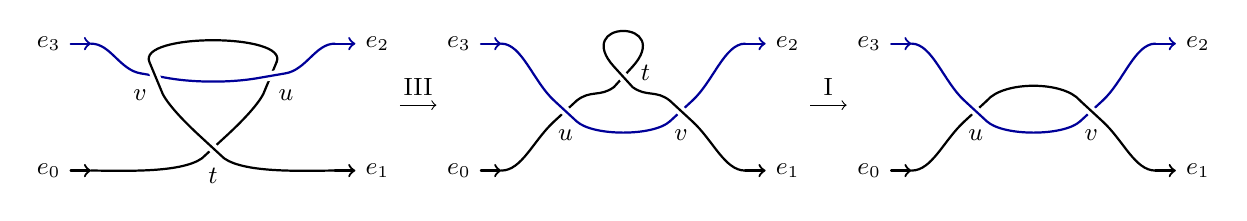
\begin{tikzpicture}[
    x=1.13cm,y=1.24cm,
    strand/.style={line width=0.8pt,line cap=round},
    a arc/.style={strand,draw=black},
    b arc/.style={strand,draw=blue!60!black},
    overpass/.style={preaction={draw=white,line width=3.4pt}},
    every node/.style={font=\small},
]
% Give ports 0 and 1 in crossing coordinates. Their opposites are 2 and 3.
\newcommand{\capports}[7]{%
  \path[shift={(#2,#3)}] (#4,#5) coordinate (#1-0)
    (#6,#7) coordinate (#1-1)
    ({-(#4)},{-(#5)}) coordinate (#1-2)
    ({-(#6)},{-(#7)}) coordinate (#1-3);
}
\newcommand{\capcrossing}[3]{%
  \draw[#2] (#1-0) -- (#1-2);
  \draw[#3,overpass] (#1-3) -- (#1-1);
}
\newcommand{\capboundary}{%
  \draw[a arc,->] (-1.60,-.65) node[left] {$e_0$} -- (-1.37,-.65);
  \draw[a arc,->] (1.37,-.65) -- (1.60,-.65) node[right] {$e_1$};
  \draw[b arc,->] (-1.60,.65) node[left] {$e_3$} -- (-1.37,.65);
  \draw[b arc,->] (1.37,.65) -- (1.60,.65) node[right] {$e_2$};
}
\newcommand{\capclaspends}{%
  \capports{u}{-.65}{-.04}{-.125}{-.105}{.125}{-.105}
  \capports{v}{.65}{-.04}{-.125}{-.105}{.125}{-.105}
  \draw[a arc] (-1.37,-.65) .. controls (-1.14,-.65) and (-1.01,-.34) .. (u-0);
  \draw[a arc] (v-1) .. controls (1.01,-.34) and (1.14,-.65) .. (1.37,-.65);
  \draw[b arc] (-1.37,.65) .. controls (-1.14,.65) and (-1.01,.26) .. (u-3);
  \draw[b arc] (v-2) .. controls (1.01,.26) and (1.14,.65) .. (1.37,.65);
  \draw[b arc] (u-1) .. controls (-.34,-.30) and (.34,-.30) .. (v-0);
}
\begin{scope}
  \capports{t}{0}{-.42}{-.125}{-.105}{.125}{-.105}
  \capports{u}{.65}{.32}{-.064}{-.14}{.16}{.025}
  \capports{v}{-.65}{.32}{-.16}{.025}{.064}{-.14}
  \capboundary
  \draw[a arc] (-1.37,-.65) .. controls (-1.03,-.65) and (-.37,-.68) .. (t-0);
  \draw[a arc] (t-2) .. controls (.36,-.12) and (.55,.07) .. (u-0);
  \draw[a arc] (u-2) .. controls (.86,.76) and (-.86,.76) .. (v-3);
  \draw[a arc] (v-1) .. controls (-.55,.07) and (-.36,-.12) .. (t-3);
  \draw[a arc] (t-1) .. controls (.37,-.68) and (1.03,-.65) .. (1.37,-.65);
  \draw[b arc] (-1.37,.65) .. controls (-1.15,.65) and (-1.05,.38) .. (v-0);
  \draw[b arc] (v-2) .. controls (-.20,.25) and (.20,.25) .. (u-3);
  \draw[b arc] (u-1) .. controls (1.05,.38) and (1.15,.65) .. (1.37,.65);
  \capcrossing{t}{a arc}{a arc}
  \capcrossing{u}{a arc}{b arc}
  \capcrossing{v}{b arc}{a arc}
  \node at (0,-.70) {$t$};
  \node at (.82,.12) {$u$};
  \node at (-.82,.12) {$v$};
\end{scope}
\draw[->] (2.10,.02) -- node[above] {$\mathrm{III}$} (2.51,.02);
\begin{scope}[xshift=5.21cm]
  \capboundary
  \capclaspends
  \capports{t}{0}{.31}{-.105}{-.105}{.105}{-.105}
  \draw[a arc] (u-2) .. controls (-.37,.18) and (-.26,.10) .. (t-0);
  \draw[a arc] (t-2) .. controls (.33,.64) and (.19,.78) .. (0,.78)
                          .. controls (-.19,.78) and (-.33,.64) .. (t-3);
  \draw[a arc] (t-1) .. controls (.26,.10) and (.37,.18) .. (v-3);
  \capcrossing{u}{a arc}{b arc}
  \capcrossing{v}{b arc}{a arc}
  \capcrossing{t}{a arc}{a arc}
  \node at (.25,.35) {$t$};
  \node at (-.65,-.29) {$u$};
  \node at (.65,-.29) {$v$};
\end{scope}
\begin{scope}[xshift=5.21cm]
  \draw[->] (2.10,.02) -- node[above] {$\mathrm{I}$} (2.51,.02);
\end{scope}
\begin{scope}[xshift=10.42cm]
  \capboundary
  \capclaspends
  \draw[a arc] (u-2) .. controls (-.34,.27) and (.34,.27) .. (v-3);
  \capcrossing{u}{a arc}{b arc}
  \capcrossing{v}{b arc}{a arc}
  \node at (-.65,-.29) {$u$};
  \node at (.65,-.29) {$v$};
\end{scope}
\end{tikzpicture}
\caption{The signed cap move. The black strand runs from \(e_0\) to
\(e_1\), and the blue strand from \(e_3\) to \(e_2\). Gaps mark the
underpasses. All crossings are positive. The type III move on
\(u,t,v\) exposes the curl at \(t\), and the type I move removes it
while fixing the four boundary endpoints.}
\label{fig:cap}
\end{figure}

Now put \(q=d-3\). At stage \(s\), for \(0\le s<q\), set
\(t=Y_{d-2-s}\). There are already \(s\) clasp pairs
\((u_j,v_j)\) for \(j<s\). Each has its two clasp edges, and
\[
       \port{v_j}1\text{--}\port{u_{j+1}}0,\qquad
       \port{v_j}2\text{--}\port{u_{j+1}}3 .
\]
The moving triangle begins at \((u_0,3),(t,2),(v_s,1)\).
At \(s=0\) the triangle and cap are in Table~\ref{tab:ladder}.
At each \(u_j\) for \(j<s\), use the first local rewrite
with \(w=v_j,\ v=v_s\). The two former attachments of \(w\)
to \(u_{j+1}\) now attach \(\port t2\) and \(\port{v_s}2\)
to \(u_{j+1}\), giving the triangle at \(u_{j+1}\).
This leaves \(\port{u_s}2\)--\(\port{v_s}3\) in place.
At \(u_s\), the cap rewrite removes \(t\) and gives the
clasp \((u_s,v_s)\).

To see the next stage, track the four ends of the unchanged
part of the ladder. At the start of stage \(s\),
\(\port t0\) is attached to \(\port{Y_{d-3-s}}2\)
and \(\port{v_s}0\) to \(\port{v_{s+1}}2\).
The first rewrite sends those attachments to \(\port{u_0}0\)
and \(\port{u_0}3\), whether it is at a clasp or at the cap.
Later moves in the stage keep them there. The cap rewires
\(\port t1\)--\(\port{u_{s+1}}0\) and
\(\port{u_s}1\)--\(\port{u_{s+1}}3\)
to the two new edges from \(\port{v_s}1,\port{v_s}2\).
The next triangle and cap therefore satisfy the same
hypotheses. This proves the induction for every \(d\).

At its end \(Y_2,\ldots,Y_{d-2}\) have been deleted.
The diagram consists of the \(d=3\) ladder with indices
\(Y_0,Y_1\) and \(u_q,u_{q+1},u_{q+2},v_q,v_{q+1},v_{q+2}\),
and \(q\) clasp pairs inserted between the two arcs
\(\port{Y_1}2\)--\(\port{u_q}0\) and
\(\port{v_q}2\)--\(\port{u_q}3\).
The first endpoint of each arc now leads into the first clasp
(or directly to \(u_q\) if \(q=0\)). The two edges
from \(v_j\) to \(u_{j+1}\) then lead to the next clasp or
to the base ladder. All other edges of the base ladder remain
as specified in the table, and the crossings of \(U\) are fixed.

\subsection{Identifying the insertion band in \texorpdfstring{\(R\)}{R}}

Number the crossings of the literal word \(R\) from zero.
Its fourth and fifth closure arcs run from \(\port{24}2\)
to \(\port 00\) and from \(\port{25}1\) to \(\port 03\).
Cut those two arcs just before crossing zero, leaving a named
incoming and outgoing end for each arc. The Reidemeister II
pairs \((6,25)\) and \((7,22)\) cancel with the four ends
open. For the first pair the bigon edges are
\(\port 60\)--\(\port{25}2,\ \port 63\)--\(\port{25}3\).
For the second they are
\(\port 72\)--\(\port{22}0,\ \port 73\)--\(\port{22}3\)
after the first cancellation. The two incoming ends and
the fourth outgoing end stay attached to their ports.
The fifth outgoing end moves from \(\port{25}1\) to
\(\port 52\). Neither cancellation meets the slab at the cut.
The resulting \(22\)-crossing projection, with the arcs
reclosed, is the \(d=3\) ladder. The port bijection has no
rotations and is given by
\[
 \begin{array}{c|ccccccccc}
 &F_j&Y_0&Y_1&u_0&u_1&u_2&v_0&v_1&v_2\\\hline
 \text{crossing of }R&8+j&23&24&0&1&2&5&4&3 .
 \end{array}
\]
This is verified by the braid port rule, including the edges
of \(U\) and the four attachments in Table~\ref{tab:ladder}.
The cut arcs correspond precisely to
\(\port{Y_1}2\)--\(\port{u_0}0\) and
\(\port{v_0}2\)--\(\port{u_0}3\).
The marked ends identify the actual fourth/fifth strand band
before the first crossing of \(R\), including both boundary
orientations. In the closed braid a positive full twist in
that band can be written at the end of \(R\).
Each clasp from the induction has the port pairing of
\(\sigma_4^2\) in this band, so the resulting projection is
the twice-reduced diagram of \(\cl{R\sigma_4^{2q}}\).
The oriented moves preserve the component containing \(U\)
and the other component. Since \(q=b-5\), this proves
Lemma~\ref{lem:isotopy}.


\begin{thebibliography}{9}
\raggedright
\bibitem{Cornwell}
C.~R. Cornwell, \emph{KCH representations, augmentations, and
\(A\)-polynomials}, J. Symplectic Geom. \textbf{15} (2017), 983--1017.
\href{https://doi.org/10.4310/JSG.2017.v15.n4.a2}{doi:10.4310/JSG.2017.v15.n4.a2}.

\bibitem{FKP}
D. Futer, E. Kalfagianni, and J.~S. Purcell, \emph{Dehn filling, volume,
and the Jones polynomial}, J. Differential Geom. \textbf{78} (2008),
429--464. \href{https://doi.org/10.4310/jdg/1207834551}{doi:10.4310/jdg/1207834551}.

\bibitem{GGLW}
H. Gao, S. Gu, Z. Li, and J. Wang, \emph{Meridional ranks of iterated
Whitehead doubles}, preprint, 2026.
\href{https://arxiv.org/abs/2611.15673v1}{arXiv:2611.15673v1}.

\bibitem{HIKMOT}
N. Hoffman, K. Ichihara, M. Kashiwagi, H. Masai, S. Oishi, and
A. Takayasu, \emph{Verified computations for hyperbolic \(3\)-manifolds},
Exp. Math. \textbf{25} (2016), 66--78.
\href{https://doi.org/10.1080/10586458.2015.1029599}{doi:10.1080/10586458.2015.1029599}.

\bibitem{Thurston}
W.~P. Thurston, \emph{The Geometry and Topology of Three-Manifolds},
Princeton lecture notes, electronic edition 1.1, 2002.
\href{https://library.slmath.org/nonmsri/gt3m/}{Electronic edition}.
\end{thebibliography}
\end{document}
